



% Use upquote if available, for straight quotes in verbatim environments
%% Options
%%%% Serif
%%%% Twocolumn
%%%%%%% Pick one of the following
%%%% numeric (numeric citation)
%%%% authordate (authordate citation)
\documentclass[serif, twocolumn, numeric, rga]{jote-article}

%\renewcommand{\paragraph}[1]{\paragraph{#1}\mbox{}\\.}

%\usepackage[backend = biber, style=numeric, citestyle = numeric, sorting=none]{biblatex}
\addbibresource{veronika.bib}

\usepackage{enumitem}% http://ctan.org/pkg/enumitem
\setlist[itemize]{noitemsep, topsep=0pt, labelindent=\parindent, leftmargin=2\parindent, label=$\triangleright$}
\setlist[description]{noitemsep, topsep=0pt}
\usepackage{pifont}
%\usepackage{amssymb}
%% Example: Using author-year citations and anonymising submission % \documentclass[blind,alpha-refs]{wiley-article}

%% Example: Using unsrtnat for numerical, in-sequence citations % \documentclass{wiley-article}
% \usepackage[numbers]{natbib}
% \bibliographystyle{unsrtnat}

%% Example: Using WileyNJD-AMA reference style and superscript %%          citations, two-column and serif fonts for AIChE % \documentclass[serif,twocolumn,lineno]{wiley-article}
% \usepackage[super]{natbib}
% \bibliographystyle{WileyNJD-AMA}
% \makeatletter % \renewcommand{\@biblabel}[1]{#1.}
% \makeatother 
% Add additional packages here if required


\usepackage{float}
\usepackage{bookmark}
\usepackage{lipsum}
% Update article type if known % Include section in journal if known, otherwise delete
\papertype{Rejected Grant Application}

\title{CrowdDetective: Wisdom of the Crowds for Detecting Abnormalities in Medical Scans}

% List abbreviations here, if any. Please note that it is preferred that abbreviations be defined at the first instance they appear in the text, rather than creating an abbreviations list.
%\abbrevs{ABC, a black cat; DEF, doesn't ever fret; GHI, goes home immediately.}

% Include full author names and degrees, when required by the journal.
% Use the \authfn to add symbols for additional footnotes and present addresses, if any. Usually start with 1 for notes about author contributions; then continuing with 2 etc if any author has a different present address.

\newbox{\myorcidaffilbox}
\sbox{\myorcidaffilbox}{\large
\includegraphics[height=1.7ex]{media/ORCIDiD_icon32x32.png}}

\author[1]{Veronika Cheplygina}
% I want to make Orcids work but thats for later \protect\href{https://orcid.org/0000-0003-0176-9324}{
\includegraphics[width=5em]{media/ORCIDiD_iconvector.pdf}}}
\authorone{Veronika Cheplygina}


%\contrib[\authfn{1}]{Equally contributing authors.}

% Include full affiliation details for all authors
\affil[1]{Medical Image Analysis, Department of Biomedical Engineering, Eindhoven University of Technology, Eindhoven, 5612 AZ, the Netherlands}
%\affil[2]{Department, Institution, City, State or Province, Postal Code, Country}

\corraddress{Veronika Cheplygina, Medical Image Analysis, Department of Biomedical Engineering, Eindhoven University of Technology, Eindhoven, 5612 AZ, the Netherlands}
\corremail{v.cheplygina@tue.nl}
\rgainfo{Netherlands Organisation for Scientific Research Veni scheme 2018}

%\presentadd[\authfn{2}]{Department, Institution, City, State or Province, Postal Code, Country}

\paperdoi{10.36850/rga1}

% Include the name of the author that should appear in the running header 
\runningauthor{Cheplygina}

\jname{Journal of Trial and Error}
\jyear{2020}
\jvolume{1}
\jissue{1}
\jpages{59--71} % To be adjusted I suppose when everything is combined
\jwebsite{https://jtrialerror.com}
\paperreceived{11 May, 2020}
\paperrevised{22 June, 2020}
% When the paper was accepted
%\paperaccepted{2 January, 2020}
\paperpublished{2 December, 2020}
\paperpublisheddate{2020-2-12}


%\jpages{1-Carbonneau2017}
\jlogo{media/jote_logo_full}

\pubpub{https://archive.jtrialerror.com/pub/crowdwisdom}



\heightabstract{60mm}
\widthaffil{55mm}

\setlength{\parskip}{0pt}


\keywordsabstract{machine learning, artificial intelligence, medical imaging, crowdsourcing, computer-aided diagnosis }

\begin{document}
\setcounter{page}{59}
\pdfbookmark[0]{Cheplygina, V.  - CrowdDetective; Wisdom of the Crowds for Detecting Abnormalities in Medical Scans}{veronikapdf}
\begin{frontmatter}
\maketitle 
\begin{abstract}
Machine learning (ML) has great potential for early diagnosis of disease from medical scans, and at times, has even been shown to outperform experts. However, ML algorithms need large amounts of annotated data -- scans with outlined abnormalities - for good performance. The time-consuming annotation process limits the progress of ML in this field.

To address the annotation problem, multiple instance learning (MIL) algorithms were proposed, which learn from scans that have been diagnosed, but not annotated in detail. Unfortunately, these algorithms are not good enough at predicting where the abnormalities are located, which is important for diagnosis and prognosis of disease. This limits the application of these algorithms in research and in clinical practice.

I propose to use the ``wisdom of the crowds'' --internet users without specific expertise -- to improve the predictions of the algorithms.
While the crowd does not have experience with medical imaging, recent studies and pilot data I collected show they can still provide useful information about the images, for example by saying whether images are visually similar or not. Such information has not been leveraged before in medical imaging applications. I will validate these methods on three challenging detection tasks in chest computed tomography, histopathology images, and endoscopy video.

Understanding how the crowd can contribute to applications that typically require expert knowledge will allow harnessing the potential of large unannotated sets of data, training more reliable algorithms, and ultimately paving the way towards using ML algorithms in clinical practice.
% Please include a maximum of seven keywords
\end{abstract}
\end{frontmatter}

\section*{Research proposal}
\vspace{\baselineskip}

\subsection*{General information}

\subsubsection*{Institution of employment at time of application}

Eindhoven University of Technology

\subsubsection*{Prospective host institution}

Eindhoven University of Technology 

\subsubsection*{Main field}

Artificial Intelligence, Expert Systems 

\subsubsection*{Other fields}

Medicine, other 

\subsubsection*{Number of words}

Description of the proposed research: 1999 (max. 2,000 words)

\noindent Knowledge utilisation: 719 (max. 750 words)

\subsection*{Description of the proposed research}


%\subsubsection*{1. Description of the proposed research}

\subsubsection*{Overall aim and key objectives}

Machine learning (ML) has seen tremendous successes in recent years, for example in classifying everyday objects such as cats in images. This progress is driven by the availability of powerful computational resources, sophisticated algorithms, but most of all, large amounts of labelled data. Data is annotated at different levels: outlining the cat in the image (a strong annotation) or tagging the whole image (a weak annotation). Strong labels are the most effective, but weak labels can also be used by weakly supervised or multiple instance learning (MIL) algorithms (Fig.\ref{fig:brain}). 

\begin{figure}
\centering 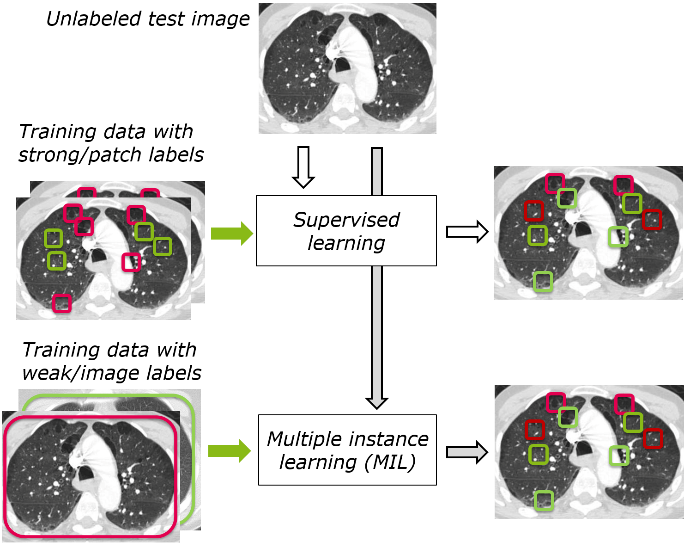
\includegraphics{articles/RGAs/Veronika/brain.png}
\caption{Supervised learning and MIL in medical imaging}
\label{fig:brain}
\end{figure}


In medicine, ML offers invaluable opportunities for diagnosis of disease, reaching expert performance \cite{Kooi2017} or even outperforming the experts \cite{Rajpurkar2017, Bejnordi2017}. However, while the amount of medical data is growing rapidly\footnote{\url{http://ec.europa.eu/eurostat/statistics-explained/index.php/Healthcare_resource_statistics_-_technical_resources_and_medical_technology}}, the data is often only weakly annotated (a scan with a diagnosis, but without outlined abnormalities). Although MIL is gaining popularity in medical imaging \cite{Manivannan2016, Cheplygina2014, Kandemir2015, Melendez2014, Cheplygina2015b, Quellec2012}, there is an overlooked, fundamental problem. MIL algorithms are optimized to predict weak annotations \cite{Quellec2017}, but the classifier best at predicting weak annotations, is often not the best at predicting strong annotations \cite{Kandemir2015, Cheplygina2015b, Vanwinckelen2016, Carbonneau2016}. In practice this means that without strong annotations, MIL algorithms are poor at localizing abnormalities \cite{Li2018}.

I propose a novel way of using crowdsourcing \cite{Howe2006} to improve the abnormality localization. Crowdsourcing is the process of gathering input by enlisting the services of a large number of people, either paid or unpaid, typically via the internet, allowing large-scale data annotation \cite{Lin2014}. A widely used example is tagging people on social media, used to improve face recognition. Crowdsourcing has therefore been successful in computer vision \cite{Lin2014, Kovashka2016} with non-expert tasks, such as recognizing everyday objects. However, internet users are not medical experts -- how could they annotate abnormalities? 
A key insight is that the crowd does not need to mimic the experts to improve MIL for detecting abnormalities. For example, for detecting abnormalities in chest CT images, I propose to instead leverage the human visual system by asking: 
\begin{itemize}
\item   To outline airways, which are easily recognizable structures (Fig.\ref{fig:airway}) 
\item   Whether patches are similar to each other 
\end{itemize}


\begin{wrapfigure}[14]{R}{0.6\columnwidth}
\vspace{-10pt}
\centering 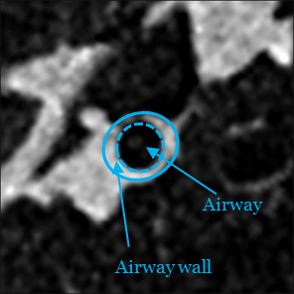
\includegraphics[width=0.6\columnwidth]{articles/RGAs/Veronika/air.png}
\caption{Airway in a chest CT patch}
\label{fig:airway}
\end{wrapfigure}

These annotations can be intuitively provided by the crowd, as demonstrated by my pilot results \cite{Cheplygina2016a, Orting2017}. Although such annotations cannot be used to directly train algorithms, they are still informative.


The visual information in these annotations can help the MIL algorithm to find better representations for the data via \emph{multi-task learning} \cite{Caruana1998a} with labels for related tasks, such as outlining airways, and with \emph{similarity-based learning} \cite{Weinberger2009, vanderMaaten2012a} with patch similarities.

The goal of this project is to improve the prediction of strong annotations by MIL, which is important for medical imaging, but also applications in other fields where annotations are scarce. Furthermore, the project will provide insight into the value of crowdsourcing in expert-level tasks. This is essential to leverage the value and scientific potential of big datasets, which are growing at an exponential rate.
\paragraph{Originality and innovative aspects.}


The problem of predicting strong labels with MIL is underexplored \cite{Quellec2017, Carbonneau2016}. Using crowdsourcing to improve MIL is novel in general - in a recent survey of crowdsourcing in computer vision \cite{Kovashka2016} none of the 195 papers address MIL, while a recent book on MIL \cite{Herrera2016a} does not mention crowdsourcing. While techniques for multi-task and similarity-based learning exist, these often have assumptions not compatible with medical images annotated by crowds. I will develop methods which better address such data.

Crowdsourcing is new to medical imaging, with most studies published in the last five years \cite{Cheplygina2016a, Maier-Hein2014, Maier-Hein2014b, Mitry2015a, Nguyen2012, Albarqouni2016}. The crowd typically mimics the experts in labelling images with a diagnosis or outlining structures in image patches, and the results are compared to expert labels. Several studies show promising results, while in other cases the crowd does not achieve the level of the experts \cite{Mitry2015a, Albarqouni2016}. Note that in most studies the crowd only labels the images -- the labelled images are then not used in ML approaches. Only \cite{Albarqouni2016} uses the labels to train algorithms, but collects labels and does not address the MIL scenario.
There is no prior work on collecting labels for related tasks and similarities, except in my recent pilot studies \cite{Cheplygina2016a, Orting2017}.

Next to my expertise in these topics I started building a community around the topic of crowdsourcing for medical imaging (\href{http://www.miccailabels.org}{MICCAI LABELS} workshop, recently funded \href{https://www.esciencecenter.nl/news/crowdsourcing-for-medical-image-analysis-wins-lorentz-escience-workshop-com}{eScience-Lorentz}
workshop), have many international collaborators and interest from industry. The project also benefits from my outreach and open science efforts (Section on Knowledge Utilisation).
\paragraph{Approach.}

I will investigate three strategies in which expert weak labels and crowd annotations can be combined to train more robust MIL algorithms: 
\begin{itemize}
\item   Experts + crowd labels for the expert task 
\item   Experts + crowd labels for related tasks 
\item   Experts + crowd similarities 
\end{itemize}

My hypothesis is the best strategy will depend on the application, as explained below.

Labels from the crowd can be combined with expert labels to create a more robust classifier by \emph{decision fusion (DF)} \cite{Kittler1998, Kuncheva2004}. In traditional DF approaches each classifier is trained on a (random) subset of the data \cite{Breiman1996a, Ho1998, Dietterich2000} -- classifiers of similar quality, and their decisions are averaged. An alternative is to weight classifiers by their estimated accuracy, which requires additional data or assumptions, such as that per image, at least half of the classifiers are correct.
This assumption may not always hold in medical images. In more difficult tasks where expert knowledge is needed, I expect that this strategy will not outperform the baseline, where the MIL algorithm is trained only on the expert weak labels.

Labels for related tasks, such as outlining airways, when the target is to detect abnormalities, can be leveraged via \emph{multi-task learning (MTL)} \cite{Caruana1998a}. The intuition is that there are underlying features helpful for both tasks, which helps to find a more robust classifier.
This is achieved by optimizing a joint loss function for the classifier.
Such approaches are used in computer vision to simultaneously detect different everyday objects in images \cite{Vezhnevets2010a}. In medical imaging MTL was used to simultaneously predict an Alzheimer's diagnosis and a cognitive test score \cite{Cheng2015}, and to simultaneously predict different abnormalities related to lung cancer \cite{Bi2008a}.

However, the computer vision approaches have assumptions that might be incompatible with medical imaging, such as well-defined boundaries for each object, and the medical imaging methods do not address MIL and expect expert labels for both tasks. I will investigate the applicability of these and similar approaches, while addressing the specifics of crowd-annotated medical images, for example, by weighting the loss function such that the expert labels are given more emphasis. I expect that the MTL strategy will be most successful when the related task is simple enough for the crowd to do, but has some relevance to the target task.

Similarities, such as ``image patch A is more similar to B than to C'' (Fig. \ref{fig:chestct}) can also add information during training. The idea is that such judgements are more intuitive for crowds to provide, even if they are not able to label the images. The similarities provide relative information about the expected classifier outputs, favouring classifiers for which these relationships hold. Examples include metric learning \cite{Weinberger2009} and similarity embedding \cite{vanderMaaten2012a, Hoffer2015a}, which I group under the name \emph{similarity-based learning} (SBL).


\begin{figure}
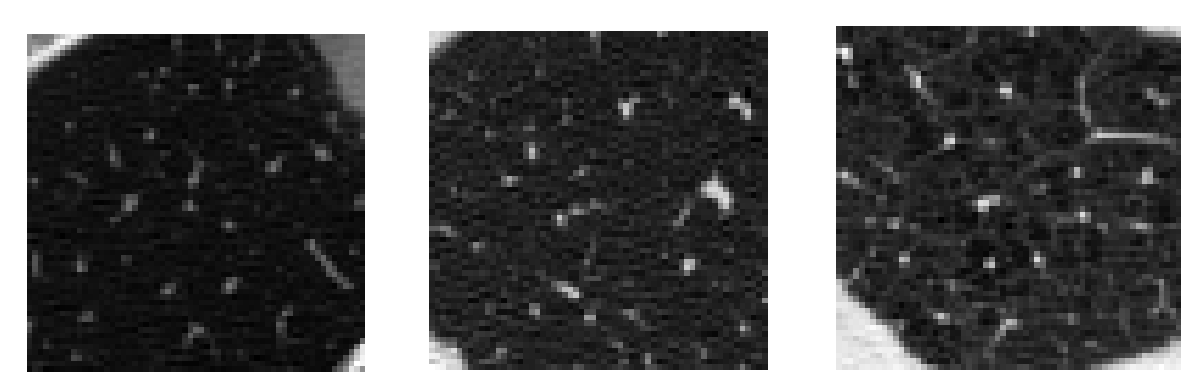
\includegraphics[width=\columnwidth]{articles/RGAs/Veronika/tissue.png}
\caption{Chest CT patches with healthy (left and middle) tissue and emphysema (right). Labelling these is difficult for non-experts, but they can still characterize the visual similarity of the patches.}
\label{fig:chestct}
\end{figure}  

Again, the assumptions of current methods that focus on MIL may not be applicable. For example \cite{Law2017} assumes that an image label can apply to at most one patch in that image, which is not true for many abnormalities. Based on my experience with different (medical and non-medical) MIL problems \cite{Cheplygina2015a, Cheplygina2016}, I will investigate how to create approaches with assumptions more suitable for medical images. I expect SBL to be successful when the crowd can focus on a single aspect of similarity, such as image texture. If there are multiple aspects to focus on, the similarities are likely to be inconsistent across annotators, and might hurt performance of MIL instead.

I will develop MIL algorithms which learn both from expert weak labels and crowd annotations, via DF, MTL or SBL. The strategies I will develop are general, therefore I will use them both with traditional \cite{Chen2006, Andrews2002} and more recent \cite{Cheplygina2016, Carbonneau2018} MIL classifiers. Similarly, the strategies will apply both to traditional features and features extracted by deep learning.

To investigate which strategy is better in which scenario, I will apply these algorithms to three applications, with different image characteristics and task difficulty: 
\begin{itemize}
\item   Localizing patches with emphysema, in chest CT images \cite{Depeursinge2012, Pedersen2009}.
  This is a task of medium difficulty, where I expect best results from   MTL because the underlying disease affects the appearance of airways,   or SBL based on recent pilot results \cite{Orting2017}.
\item   Localizing different surgical instruments in endoscopy videos   \cite{Ross2017}. This is a relatively easy task where DF is already likely to   be successful.
\item   Localizing cancerous regions in histopathology images \cite{Veta2015}. This   is a difficult task, where I would expect best results for SBL, or MTL   if a simple but powerful related task can be defined in collaboration   with experts.
\end{itemize}

The datasets have expert weak labels, but also some expert strong labels available, which I will use for validation purposes. I will collect annotations via two platforms, with different trade-off between collection time and quality \cite{Mao2013}: 
\begin{itemize}
\item   \href{https://www.mturk.com/mturk/welcome}{Amazon Mechanical Turk}
  with paid crowds, which reduces the time to 1-Rajpurkar2017 days, but could reduce   quality.
\item   \href{https://www.zooniverse.org/}{Zooniverse} with unpaid volunteers   interested in science, which increases time, but also quality.
\end{itemize}


\begin{wrapfigure}{R}{0.6\columnwidth}
\vskip-12pt
\centering 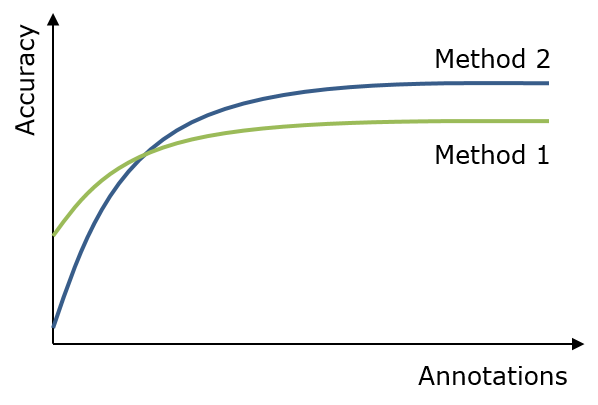
\includegraphics[width=0.6\columnwidth]{articles/RGAs/Veronika/graph.png}
\caption{Learning curves, method 1 is better with few annotations and vice versa.}
\label{fig:graph}
\end{wrapfigure}

The next step is to decide which patches to annotate and how many annotators to assign to each patch. Combining annotators increases the quality but, given the same budget, decreases the total amount of annotated data. Because ML (and thus also MIL) algorithms benefit from seeing a larger set of data and my goal is not to produce expert-quality annotations, I expect it will be more valuable to maximize the amount of annotated patches. To keep the number of annotations within budget, I will investigate active selection of patches, for example based on their uncertainty or diversity according to the MIL algorithm.




Lastly I will compare the strategies to baselines, such as training MIL only with expert weak labels, and to each other. In this process I will vary the number of expert labels and crowd annotations used, in order to create more scenarios than the three applications investigated.

By analysing these results from three different applications, I will aim to extract general rules on when each strategy is best to use.

\subsubsection*{Research plan}

The project has four work packages: 
\begin{description}
\item WP1: Decision fusion with labels 
\item WP2: Multi-task learning with related labels 
\item WP3: Representation learning with similarities 
\item WP4: Generalization 
\end{description}

In WP1-WP3, I will crowdsource the corresponding type of annotations and develop MIL algorithms for combining these annotations with expert weak labels. The deliverables are extended versions of my publicly available MIL toolbox \cite{Tax2016} and papers published in high impact conferences and journals. In WP4 I will compare the strategies and draw up recommendations for their use. The deliverable is a paper with a related blog post.

% Please add the following required packages to your document preamble:
% \usepackage{booktabs}
% \usepackage[table,xcdraw]{xcolor}
% If you use beamer only pass "xcolor=table" option, i.e. \documentclass[xcolor=table]{beamer}
\begin{table*}
\sffamily
\centering
\setlength{\extrarowheight}{0pt}
\addtolength{\extrarowheight}{\aboverulesep}
\addtolength{\extrarowheight}{\belowrulesep}
\setlength{\aboverulesep}{0pt}
\setlength{\belowrulesep}{0pt}
\begin{tabular}{@{}p{27mm}>{\centering\arraybackslash}p{8mm}>{\centering\arraybackslash}p{8mm}>{\centering\arraybackslash}p{8mm}>{\centering\arraybackslash}p{8mm}>{\centering\arraybackslash}p{8mm}>{\centering\arraybackslash}p{8mm}>{\centering\arraybackslash}p{9mm}>{\centering\arraybackslash}p{8mm}>{\centering\arraybackslash}p{8mm}>{\centering\arraybackslash}p{8mm}>{\centering\arraybackslash}p{7mm}>{\centering\arraybackslash}p{7mm}} 
\toprule
 & \textbf{Y1 }                                  &                                      &                                      &                                      & \textbf{Y2 }                                  &                                      &                                      &                                      &\textbf{ Y3    }                               &                                      &                                      &                                       \\ \midrule 
WP1                                & {\cellcolor{jote}} & {\cellcolor{jote}} & {\cellcolor{jote}} & {\cellcolor{jote}} &                                      &                                      &                                      &                                      &                                      &                                      &                                      &                                       \\ 
WP2                                &                                      &                                      &                                      & {\cellcolor{jote}} & {\cellcolor{jote}} & {\cellcolor{jote}} & {\cellcolor{jote}} &                                      &                                      &                                      &                                      &                                       \\ 
WP3                                &                                      &                                      &                                      &                                      &                                      &                                      & {\cellcolor{jote}} & {\cellcolor{jote}} & {\cellcolor{jote}} & {\cellcolor{jote}} &                                      &                                       \\ 
WP4                                &                                      &                                      &                                      &                                      &                                      &                                      &                                      &                                      &                                      & {\cellcolor{jote}} & {\cellcolor{jote}} & {\cellcolor{jote}}  \\ 
Knowledge utilization (next section) & UM                                   & Visit DKFZ                           &                                      &                                      & UM                                   & Visit ETS                            & \!\!\!Workshop                             &                                      & UM                                   &                                      & \multicolumn{2}{l}{Lectures}                                                \\
\bottomrule
\end{tabular}
\caption{Time Plan. UM = user meeting}
\label{tab:schedule}
\end{table*}


I will conduct the research at the
\href{https://www.tue.nl/en/university/departments/biomedical-engineering/research/research-groups/medical-image-analysis/}{Medical Image Analysis group}, TU/e. The main collaborators (I will visit both for 3 months are

\begin{itemize}
\item   \href{https://www.dkfz.de/en/cami/team/people/Lena_Maier-Hein.html}{Prof.  Lena Maier-Hein} (DKFZ, Germany). I will collaborate with her on crowdsourcing aspects, and apply my algorithms to endoscopy video   data from her group.
\item   \href{http://etsmtl.ca/Professeurs/egranger/Accueil?lang=en-CA}{Prof.  Eric Granger} (ETS, Canada) and
  \href{https://mcgillgcrc.com/research/members/mccaffrey}{Dr.  Luke McCaffrey} (McGill, Canada). I will collaborate with   Prof. Granger on MIL and apply my algorithms to histopathology data   provided by Dr. McCaffrey.
\end{itemize}
I also have contacts in medical imaging and crowdsourcing communities whom I could approach for advice, including Dr. Marleen de Bruijne (Erasmus MC), Dr. Javed Khan (TU/e), Dr. Alessandro Bozzon (TU Delft).

\subsection*{Knowledge utilisation}

\subsubsection*{Potential}

\paragraph{Research.}

\noindent In medical imaging the results of my research will be beneficial to many research groups, as the annotation problem is present in many different applications. In machine learning (ML) the research will demonstrate the potential of improving algorithms with crowd annotations which are not typically leveraged. This is an underexplored area, but is likely to spark interest in the community. I expect this to assist in development of (general purpose) algorithms focusing on such annotations.

Furthermore I expect interest from other applications where annotated data is scarce, such as remote sensing \cite{Fritz2009} and ecology \cite{Fink2014}.
Lastly, the behaviour of the crowd (who contributed what and why) could be of interest to research groups in human-computer interaction \cite{Mao2013}
and social sciences.

\paragraph{Industry.} 

\noindent There is already great interest from the industry in ML, and medical imaging is catching up, for example in 2017 the leading conference \href{http://www.miccai2017.org/partners}{MICCAI} had IBM, Nvidia, Siemens and many medical imaging startups as sponsors.

The interest in my project is demonstrated by the companies in Table \ref{tab:usergroup}, including IBM Research. These companies could integrate the research outcomes in their products, which are designed to be user-friendly and secure. This will enable translation of the proposed research to products and (in case of medical imaging) the clinic.

\paragraph{Society.}

\noindent The research area is relevant to several questions on the National Science Agenda, including health (questions \href{https://vragen.wetenschapsagenda.nl/cluster/hoe-kunnen-big-data-en-technologische-innovatie-e-health-bijdragen-in-de-zorg}{105}, \href{https://vragen.wetenschapsagenda.nl/cluster/hoe-kunnen-we-longziekten-beter-begrijpen-en-behandelen}{89}, \href{https://vragen.wetenschapsagenda.nl/cluster/hoe-maken-we-de-gezondheidszorg-kwalitatief-zo-goed-mogelijk-en-houden-we-haar-betaalbaar}{94}) and society and technology (\href{https://vragen.wetenschapsagenda.nl/cluster/big-data-kunnen-we-grote-datasets-en-het-verzamelen-daarvan-benutten-voor-het-realiseren-van}{112}, \href{https://vragen.wetenschapsagenda.nl/cluster/welke-sociale-veranderingen-als-gevolg-van-technologische-veranderingen-zijn-aanstaande-en}{108}).
In health, there are long term benefits of improved medical imaging algorithms, such as better prognosis and diagnosis of disease, and better use of the experts' time.

For society, there are benefits in involving the public as annotators, which can raise awareness about health. In the long term, contributing to such projects could create jobs or volunteering opportunities, accessible to people who are be unable to work due to health or care responsibilities \cite{Hara2018}, increasing their well-being.

\subsubsection*{{\large Implementation}}

\paragraph{Research.}

\noindent I will publish in relevant venues (MICCAI, Pattern Recognition) and make the papers/data/code available online. I will continue organizing events I'm already involved in (MICCAI LABELS, eScience-Lorentz workshop, NVPHBV) and giving talks about my work. In years 1 and 2 my research visits to Germany and Canada will help in reaching other groups I am not yet in contact with. I expect other groups will use my methods for their data from the first year of the project.

In year 2 I will organize a workshop on the intersection of ML and crowdsourcing in label-scarce applications beyond medical imaging. I will invite researchers via my network and online communities I'm a member of (\href{https://groups.google.com/forum/\#!forum/ml-news}{ml-news}, \href{https://groups.google.com/forum/\#!forum/crowd-hcomp}{crowd-hcomp}).
The impact is more difficult to predict, but I expect that at least some groups will be interested in either the data and/or code generated by my project, and translating these to their own applications.

\paragraph{Industry.}

\noindent I have established a user group (Table \ref{tab:usergroup}) of industry representatives interested in the research outcomes. I will organize meetings with this group \textbf{every year}. Translation to industry could start within 2-Cheplygina2013 years of starting the project. This collaboration could lead to other joint projects, ensuring impact even after completion of the current research.



\begin{table}[h]\sffamily
\begin{tabular}{p{0.13\columnwidth}p{0.17\columnwidth}p{0.55\columnwidth}}
\toprule
\textbf{Group}   & \textbf{Contact}   & \textbf{Role}                                                                                                                                                                                           \\ \midrule
IBM Research     & (anonymized)   & IBM Research is working on a crowdsourcing solution for “internal crowds” (e.g. colleagues) and is interested in a medical imaging application.                                                         \\
Thirona, ClinicalGraphics        & (anonymized)   & Thirona and ClinicalGraphics develop software for medical imaging. They train employees for annotating images, and want to scale up the annotations without an equal increase in cost. \\
Cosmonio         & (anonymized) & Cosmonio develops an app that allows interaction between the medical expert and the algorithm. My research will help to optimize the type of interactions needed.                                       \\ \bottomrule
\end{tabular}
\caption{User Group}
\label{tab:usergroup}
\vspace{-\baselineskip}
\end{table}

\paragraph{Society.}

I will reach a broader group of people (people with an interest in science and/or annotators from AmazonMT and ZooUniverse platforms) via outreach through my blog (3K visits per month) and Twitter (1.8K followers). I will blog about my project \textbf{every quarter}, explaining my project to an audience interested in science, but without a technical background.

In \textbf{year 3} I will record lectures for an online course on \href{http://www.datacamp.com}{DataCamp}\footnote{The author now distances herself from this company. She would not use   their software after an investigation has shown an incident of sexual   misconduct from the former CEO and the ensuing mismanagement of this   incident. For transparency, the editors are maintaining the company   name.}, where I am already setting up an image analysis course. The course will combine machine learning, medical imaging and crowdsourcing, but will not require technical prerequisites. This is a more long-term strategy than the others.


\subsection*{Cost estimates}
\begin{table}[h] \sffamily
\begin{tabular}{lp{0.11\columnwidth}p{0.19\columnwidth}p{0.1\columnwidth}l}
\toprule
       & Personnel & Communication\footnotemark & Teaching & Equipment/ Material \\ \midrule
Year 1 & 73.000    & 4.000 &          & 5.000              \\
Year 2 & 75.400    & 5.000  &          & 3.000              \\
Year 3 & 77.700    & 2.000  & 2.000    & 1.900              \\
Total  & 226.100   & 11.000 &          & 9.000             \\ \bottomrule
\end{tabular}
\caption{Cost Estimates}
\label{tab:table4}
\vspace{-\baselineskip}
\end{table}

\footnotetext{Conferences, outreach, publication, and travel}

\subsubsection*{Total budget requested}

€250.000 

\subsubsection*{Intended starting date}

September 1, 2018 
\subsubsection*{Application for additional grants}

No 
\subsection*{Data management plan}

\subsubsection*{Will data be collected or generated that are suitable for reuse?}

Yes. I will collect annotations (labels and similarities) for patches extracted from already available medical images. The annotations will be stored in the widely reusable JSON format.

I will also generate features -- numerical data which describes the images, but from which the images cannot be reconstructed. The features will be stored as CSV files to facilitate reuse across different platforms.

The annotations and features (\emph{hereafter referred to as relevant data}) can be reused in development of other machine learning algorithms.

\subsubsection*{Where will the data be stored during the research?}

All data is stored electronically. The annotations will be collected via the cloud (Amazon Mechanical Turk or Zooniverse) and thus a secure back-up will always be available. The annotations will then be copied to secure network drives available at the host institute. This is also where the generated features will be stored. Daily back-ups are made on this storage facility.

Upon publication of a paper, I will also upload the relevant data to the \href{http://www.figshare.com}{Figshare} repository (see below).

\subsubsection*{After the project has been completed, how will the data be stored for the long-term and made available for the use by third parties? To whom will the data be accessible?}

I will store the relevant data on \href{http://www.figshare.com}{Figshare} which will ensure its long-term preservation. Figshare has agreements with publishers such as Nature, PLOS, and others to ensure the data persists for a minimum of 10 years.
I will share the relevant data under the Creative Commons Attribution-NonCommercial-ShareAlike (CC-BY-NC-SA) license.

\subsubsection*{Which facilities (ICT, (secure) archive, refrigerators or legal expertise) do you expect will be needed for the storage of data during the research and after the research? Are these available?*}

\emph{*ICT facilities for data storage are considered to be resources such as data storage capacity, bandwidth for data transport and calculating power for data processing.}

I will use in-house computing facilities, which are already available at the host institute.

\subsection*{Ethics}

\subsubsection*{Use of extension clause}

No 
\subsubsection*{Ethical aspects}


\begin{table}[h!]\sffamily\mdseries\begin{tabularx}{\columnwidth}{Xl}\toprule 
Approval from a recognised (medical) ethics review committee & Not applicable \tabularnewline Approval from an animal experiments committee & Not applicable\tabularnewline Permission for research with the population screening Act & Not applicable \tabularnewline \bottomrule
\end{tabularx}
\caption{Ethical aspects}
\vspace{-\baselineskip}
\end{table}



\paragraph{Declarations.}

By submitting this form I endorse the code of conduct for laboratory animals and the code of conduct for biosecurity/possibility for dual use of the expected results and will act accordingly if applicable.
\begin{itemize}
\item[\checkedbox] I have completed this form truthfully.

\item[\checkedbox] By submitting this document I declare that I satisfy the nationally and internationally accepted standards for scientific conduct as stated in the \emph{Netherlands Code of Conduct for Scientific Practice} \emph{2014} (Association of Universities in the Netherlands) 
\item[$\square$] I have submitted non-referees. 
\end{itemize}

\noindent\paragraph{Name:} Veronika Cheplygina

\noindent\paragraph{Place:} Eindhoven

\noindent\paragraph{Date:} 8 January 2018

\subsection*{Society}

\subsubsection*{Public summary}

\paragraph{Crowds as medical detectives (ENG).} 

\noindent\emph{Dr.ir. V. (Veronika) Cheplygina (v), TU/e -- Computer Science}

Detecting abnormalities in medical images is essential for diagnosis and treatment of illness. Computer algorithms can learn to do this using manually annotated scans, but the annotation process is costly for experts. This project studies how annotations made by untrained internet users can improve the detection accuracy of computer algorithms.

\paragraph{Internetgebruikers als medische experts? (NL).} 

\noindent\emph{Dr.ir. V. (Veronika) Cheplygina (v), TU/e -- Informatica}

Het detecteren van afwijkingen in medische scans is belangrijk voor diagnose en behandeling van de ziekte. Computeralgoritmes kunnen dit leren van handmatig geannoteerde beelden, maar dit kost experts veel tijd. Dit project onderzoekt hoe annotaties van gewone internetgebruikers de automatische detectie van afwijkingen kunnen verbeteren.

\section*{Reviews}

\subsubsection*{Grant}
Vernieuwingsimpuls Veni ENW 2018

\subsubsection*{Title}
CrowdDetective: wisdom of the crowds for detecting abnormalities in medical scans

\subsubsection*{Applicant}
Dr. ir. V.V. Cheplygina

\subsubsection*{File number}
016.Veni.192.066

\noindent \textit{Your rebuttal on the referee reports is in progress}

\phantomsection \addcontentsline{toc}{subsection}{Referee report of referee 1}\subsection*{Referee report of referee 1} 

\subsubsection*{Assessment of the quality of the researcher.}
\paragraph{Explanation.}

Criteria - Quality of the researcher:
\begin{itemize}
    \item in terms of profile fit in the target group;
 \item from an international perspective belongs to the 10 to 20\% of his/her peer group;
 \item academic excellence as demonstrated by the PhD thesis, publications and/or other relevant achievements in the field 
    \item inspiring enthusiasm for research and/or technology;
 \item persuasiveness;
 \item clear indications of an outstanding talent for academic research. 
\end{itemize}

The Veni scheme aims at outstanding researchers only: the top 10-20\% of his/her international peer group.

\paragraph{Question a:}
\textit{What is your opinion on the past performance of the researcher (as demonstrated by his/her doctoral thesis, publications, and other relevant scientific achievements)?}

\paragraph{Comments:}

The applicant shows a clear focus in her research on multiple instance learning (MIL), one of the key components of the present application. She has several years of postdoctoral experience dealing with the application of MIL related algorithms to tasks in medical image analysis. I see some publications in journals, such as Pattern recognition and Pattern recognition letters, one Miccai paper. She has co-organized a workshop at the same conference, dealing with data annotation and crowd sourcing, the other key component of the present application. She also organized a workshop at ICML, and lists several international research visits. After only two years of national postdoc experience, she became assistant professor.

Overall, the applicant presents herself with a profile dedicated to an academic career, a driving research interest, all aligned well with the present research proposal. As a minor grain of salt I would have hoped for (more) high impact publications, i.e., either highly cited papers (and 8 years after the MSc there may be one or two highly cited papers, whatever the journal or conference), or contributions to high visibility conferences, such as ICML, NIPS, CVPR, or a second or third MICCAI paper.

\paragraph{Question b:}
\textit{Does the applicant belong to the top 10-20\% of his/her international peer group? Which scientific achievements or talents of the applicant show he/she belongs to this top?}

\paragraph{Comments:}

I see a number of activities, such as international collaborations and research visits, co-organization of events and workshops that actively shape the discussion of the research community. She actively disseminates research ideas via new media with followers being interested in her views and opinions. I think this does set her apart from many of her peers. There are some noticeable publications, although with a 5 year PhD and 3 years of postdoc (and assistant professor) level research, a number of other researchers in the field might have a stronger publication record. Depending on how to weigh both aspects she may be among the top 20\% of her peers.

\subsubsection*{Assessment of the quality, innovative character and academic impact of the proposal}

\paragraph{Explanation.}

Criteria - Quality, innovative character and academic impact of the proposed research 
\begin{itemize}\item challenging in terms of content; \item originality of the research topic; \item innovative scientific elements; \item potential to make an important contribution to science; \item effective in terms of proposed methodology.
\end{itemize}

\paragraph{Question a:}
\textit{Please comment on the relevance of the problem and on the originality and challenging content of the proposal.}

\paragraph{Comments:}

The problem of how to include crowd-sourced expert and non expert annotations is a relevant problem in machine learning and, hence, in medical image processing research. The problem is not solved yet and any solution would have the potential to impact significantly on the design and dissemination of machine learning in diagnostic clinical image analysis. Still, the proposed project could be stronger if it would not only focus on the comparison of different (more or less) existing techniques to a few selected (and more or less well defined) problems, but would promise to contribute to the advancement of related machine learning algorithms itself. I would see that generating these algorithms may be a natural second step, but - as it is - the application only promises to "investigate three strategies" that are likely to be data set dependent (as the applicant suggests). Overall, I feel the application promises to deliver solid and systematic research that, however, is far from offering new innovative concepts and contributions to the field.

\paragraph{Question b:}
\textit{What are the innovative aspects of the proposal? Will the research break new ground by generating new concepts, a deeper understanding, new methods, etc.?}

\paragraph{Comments:}

The main contribution will be a systematic comparison of different analytic strategies on different data sets. As such, it promises some 'best practice' guidance in a field that would, indeed, would benefit from such systematic research.

\paragraph{Question c:}
\textit{What is your opinion on its potential to make a major contribution to the advancement of scholarship, science or technology (academic impact)?}

\paragraph{Comments:}

see 2.b)

\paragraph{Question d:}
\textit{To what extent is the proposed method effective? Please comment.}

\paragraph{Comments:}

The research strategy is well described, and the aims the applicant is presenting are likely to be reached.

\phantomsection \addcontentsline{toc}{subsubsection}{Assessment of the knowledge utilisation}\subsubsection*{Assessment of the knowledge utilisation} 

\paragraph{Explanation.}

Criteria - Knowledge utilisation (= KU) 

NWO uses a broad definition of KU: not only innovative end of pipe product creation is considered, but also purposeful interaction with (potential) knowledge users, such as industry or public organisations and knowledge transfer to other scientific disciplines. NWO asks applicants to fill out the paragraph on KU. An applicant may however explain that KU cannot be expected given the nature of the research project. In that case, we still kindly ask you to assess whether the applicant has provided reasonable argument or evidence sufficiently. 

\noindent Potential: \begin{itemize} \item contribution to society and/or other academic areas; \item disciplines and organisations that might benefit from the results. \end{itemize}
Implementation: \begin{itemize} \item action plan to allow the outcomes of the research project to benefit the potential knowledge users; \item if and how the potential knowledge users will be involved; \item (concrete) outcomes for society; \item the period over which KU is expected to occur.\end{itemize}

\paragraph{Question a:}
\textit{What is your opinion on the described relevance of the results of the research?}

\paragraph{Comments:}

In the best case the project will help paving the road for simplifying research in medical image computing and the translation of medical image computing technology into clinical practice. The outcome of the project, i.e., a description of the optimal strategy for structing diagnostic information linked to a given medical image set, can be used both in the design, or evaluation, or continuous quality control of these technologies. As such, i would consider the overall research direction to be interesting and relevant also from a wider perspective.

\paragraph{Question b:}
\textit{Please comment on the effectiveness and feasibility of the proposed approach for knowledge utilisation.}

\paragraph{Comments:}

Data sets and best practice recommendations, together with related algorithms, will be the promised output: "By analysing these results from three different applications, I will aim to extract general rules on when each strategy is best to use". Whether these general rules exist, will only be know upon completion of the projection. I am somewhat missing a 'basic methodological research' component in the research objectives, for example, exploring one particular machine learning algorithm for MIL on top of the promised systematic comparison (whether this is the ubiquitous deep learning or any other). Similarly, a 'driving clinical problem' that would be solved at the end of the project, would have been nice as well (e.g., new solutions to one interesting problem that would be relevant - whether these rules generalize to other tasks, or not).

\paragraph{Question c:}
\textit{Only answer this question in case the applicant argued that knowledge utilisation is not to be expected given the nature of the research proposal: Does the applicant convincingly explain why knowledge utilisation is not applicable for his/her research project (see also the information under criterion 3 listed above)?}

\paragraph{Comments:}

Knowledge Utilization is expected.

\phantomsection \addcontentsline{toc}{subsubsection}{Final assessment}\subsubsection*{Final assessment} 

\paragraph{Question a:}
\textit{How do you assess the entire application? Please give your final scoring (A+/A/B/UF/U).}

\paragraph{Comments:}

03, B

\paragraph{Question b:}
\textit{Could you please summarize (point by point) the strengths and weaknesses of the grant application focussing on the candidate, proposal and knowledge utilisation?}
\paragraph{Comments:}
The applicant presents herself with a dedicated and good career path in medical image computing. There is a focus on MIL, that is relevant for the present project, although I feel that publications are cited for systematic comparisons, benchmarks, and implementations than for innovative methodological contributions. The proposed project is very timely and, in case "general rules" can be found, has the potential to have significant impact. It promises these contributions from a systematic study, rather than from new innovative concepts and ideas.

\phantomsection \addcontentsline{toc}{subsubsection}{Feedback datamanagement}\subsubsection*{Feedback datamanagement} 
\paragraph{Question.}
Feedback datamanagement
\paragraph{Comments:}
no

\phantomsection \addcontentsline{toc}{subsection}{Referee report of referee 2}\subsection*{Referee report of referee 2} 

\subsubsection*{Assessment of the quality of the researcher.}
\paragraph{Explanation.}
Criteria - Quality of the researcher:
\begin{itemize}
    \item in terms of profile fit in the target group;
 \item from an international perspective belongs to the 10 to 20\% of his/her peer group;
 \item academic excellence as demonstrated by the PhD thesis, publications and/or other relevant achievements in the field 
    \item inspiring enthusiasm for research and/or technology;
 \item persuasiveness;
 \item clear indications of an outstanding talent for academic research. 
\end{itemize}
\paragraph{Question a:}
\textit{What is your opinion on the past performance of the researcher (as demonstrated by his/her doctoral thesis, publications, and other relevant scientific achievements)?}
\paragraph{Comments:}
The researcher has a very good profile, with organising of workshops and interesting publications in good venues. It is a junior researcher so major impact in terms of citations can not be expected. The research direction is in line with her previous work and she has experience with research visits as well.
\paragraph{Question b:}
\textit{Does the applicant belong to the top 10-20\% of his/her international peer group? Which scientific achievements or talents of the applicant show he/she belongs to this top?}
\paragraph{Comments:}
She has received recognition by being part of the workshop organisers at LABELs and has had several interesting publications.

\subsubsection*{Assessment of the quality, innovative character and academic impact of the proposal}
\paragraph{Explanation.}
Criteria - Quality, innovative character and academic impact of the proposed research 
\begin{itemize}\item challenging in terms of content; \item originality of the research topic; \item innovative scientific elements; \item potential to make an important contribution to science; \item effective in terms of proposed methodology.
\end{itemize}
\paragraph{Question a:}
\textit{Please comment on the relevance of the problem and on the originality and challenging content of the proposal.}
\paragraph{Comments:}
The problem of limited annotation is an important problem in medical image analysis and a major limiting factor of machine learning in image analysis. Another important factor is the amount of data available, which increasingly gets easier with large repositories such as TCIA and TCGA that were not even mentioned in the text.
\paragraph{Question b:}
\textit{What are the innovative aspects of the proposal? Will the research break new ground by generating new concepts, a deeper understanding, new methods, etc.?}
\paragraph{Comments:}
Using Crowdsourcing has been done many times in medical image analysis and a few examples are mentioned. The link of weak annotations is somewhat novel but it seems that there are other approaches that would need to be combined. Just getting more data is often not enough and getting the right images annotated, so those that are on the decision boundaries would seem most important. I did not see any strategy of quality control of the crowdsourced annotations and this seems like the major factor that is important.
\paragraph{Question c:}
\textit{What is your opinion on its potential to make a major contribution to the advancement of scholarship, science or technology (academic impact)?}
\paragraph{Comments:}
There is an opportunity to advance the area medical image annotation but to a limited degree with the approaches give if no quality control is done ad if only weak labels are given.MIL is important and finding a link between the annotation and the best approaches could be very interesting.

Pretty much all medical images have reports associated to them, so ignoring the available weak labels would be a pity.

These can be radiology and pathology reports and may be more effective than getting labels of limited quality.
\paragraph{Question d:}
\textit{To what extent is the proposed method effective? Please comment.}
\paragraph{Comments:}
It is very hard to judge if the method will work. Some approaches haven been using crowdsourcing in the past and they show that with strong quality control this works well. It is not clear how this will be leveraged by the proposed approached.

\phantomsection \addcontentsline{toc}{subsubsection}{Assessment of the knowledge utilisation}\subsubsection*{Assessment of the knowledge utilisation} 
\paragraph{Explanation.}
Criteria - Knowledge utilisation (= KU) 

NWO uses a broad definition of KU: not only innovative end of pipe product creation is considered, but also purposeful interaction with (potential) knowledge users, such as industry or public organisations and knowledge transfer to other scientific disciplines. NWO asks applicants to fill out the paragraph on KU. An applicant may however explain that KU cannot be expected given the nature of the research project. In that case, we still kindly ask you to assess whether the applicant has provided reasonable argument or evidence sufficiently. 

\noindent Potential: \begin{itemize} \item contribution to society and/or other academic areas; \item disciplines and organisations that might benefit from the results. \end{itemize}
Implementation: \begin{itemize} \item action plan to allow the outcomes of the research project to benefit the potential knowledge users; \item if and how the potential knowledge users will be involved; \item (concrete) outcomes for society; \item the period over which KU is expected to occur.\end{itemize}
\paragraph{Question a:}
\textit{What is your opinion on the described relevance of the results of the research?}
\paragraph{Comments:}
The results have a potential to increase clinical decision making if it is working well. Still, all relies on the techniques to work and the annotation to be of good quality and there are currently no methods for quality control, so this is somewhat limited.
\paragraph{Question b:}
\textit{Please comment on the effectiveness and feasibility of the proposed approach for knowledge utilisation.}
\paragraph{Comments:}
The research proposes contact with industry and has an industrial panel. It is not clear how exactly the interaction will be done and how intellectual property rights can be shared. AI in medicine is a hot topic in industry as well, so there definitely is potential if things work well.
\paragraph{Question c:}
\textit{Only answer this question in case the applicant argued that knowledge utilisation is not to be expected given the nature of the research proposal: Does the applicant convincingly explain why knowledge utilisation is not applicable for his/her research project (see also the information under criterion 3 listed above)?}
\paragraph{Comments:}
knowledge utilisation is expected.

\phantomsection \addcontentsline{toc}{subsubsection}{Final assessment}\subsubsection*{Final assessment} 
\paragraph{Question a:}
\textit{How do you assess the entire application? Please give your final scoring (A+/A/B/UF/U).}
\paragraph{Comments referee.}
03, B
\paragraph{Question b:}
\textit{Could you please summarize (point by point) the strengths and weaknesses of the grant application focussing on the candidate, proposal and knowledge utilisation?}
\paragraph{Comments:}
\subparagraph{Strong points:}
\begin{itemize}
\item important domain of medical data annotation to train machine learning classifiers

\item crowdsourcing has shown strong potential with good quality control

\item good links with the MICCAI community via the LABELS workshop

\item good to adapt machine learning to specific types of annotations
\end{itemize}

\subparagraph{Weak points:} 
\begin{itemize}
    \item  quality control is not mentioned and this seems essential

\item active learning, so selecting the best images to annotate with maximised information gain is not mentioned

\item there are many more papers suing crowdsourcing for medical imaging than mentioned and the background should really be checked

\item existing large data repositories are not mentioned such as TCGA and TCIA

\item why are expert labels not used to control crowd labels? Why would combinations be useful? If expert labels exist than crowd labels do not seem necessary

\item the similarity between images or patches extremely subjective and texture is not a concept where people will have consistent answers; there is much literature on subjective perception and non of it is mentioned

\item it is not clear which images are annotated and how many images are needed; who will provide images? who will test the system?
\end{itemize}
\phantomsection \addcontentsline{toc}{subsubsection}{Feedback datamanagement}\subsubsection*{Feedback datamanagement} 
\paragraph{Question.}
Feedback datamanagement
\paragraph{Comments:}
The data management only concentrates on the annotations to be collected and not on the raw data. Where will the images originate from? How many are available? Who will test the algorithm and who will generate the ground truth? Is ethics approval for the CT and histopathology images available? By whom? How will it be insured that these data are treated properly? These are human data!

Sharing only annotations without the raw data would have a very limited usefulness.


\section*{Rebuttal}
\phantomsection \addcontentsline{toc}{subsubsection}{File number}\subsubsection*{File number} 
016.Veni.192.066
\phantomsection \addcontentsline{toc}{subsubsection}{Name of candidate}\subsubsection*{Name of candidate} 
Veronika Cheplygina
\phantomsection \addcontentsline{toc}{subsubsection}{Title}\subsubsection*{Title} 
CrowdDetective: wisdom of the crowds for detecting abnormalities in medical scans
\vskip5pt
\noindent I would like to start by thanking the committee and the reviewers for taking the time to provide feedback on my application. Below I first address the overall opinion of the reviewers and then discuss a few specific points. Direct quotes from the reviewers are in \textit{\textcolor{red}{red}}, and direct quotes from my proposal are in \textit{\textcolor{jotedark}{blue}}. The page numbers refer to pages in my submitted PDF, where my research proposal is on pages 4 through 9.

The reviewers are positive about my profile as researcher, mentioning important publications and my leadership role in the community around my research topic. R1 comments that my publication record could have been stronger. I would disagree with this, since several of my publications have been cited at 5 or 10 times the impact factor of the venue. Furthermore, since submitting the Veni, my citations increased from 230 to 254, and my h-index from 9 to 10. Two papers I published in 2017 already have 6 and 4 citations, therefore I would expect the h-index to further increase 12 in 2018. This is exceptional for somebody at my career stage, after 6.5 years in total (not 8, as the reviewer calculated) spent on research.

The reviewers agree that the problem is important, the method has potential and describe the project as well-defined. R1 is concerned with a more innovative contribution of the project, and suggests it would have been better to focus on one specific MIL algorithm, AND on one clinical problem. First, a key innovation of the proposal is to focus on different types of annotations that have been collected from the crowd, which has not been addressed before in medical imaging. Furthermore, I have specifically chosen to focus on a range of methods and applications, providing general guidelines for the field. I would argue that this is more innovative than developing specific methods for specific applications, which is what is regularly being done at most conferences on the topic.

In contrast to R1, R2 seems to find the proposal too innovative, and suggests it would be better to follow the existing approach – collecting labels from the crowd, and comparing them to expert labels. As I discuss in the proposal, this is likely not to be an optimal strategy. My proposed methods, which focus on alternative (not yet investigated) types of annotations, are more promising in this regard. Since they rely on more intuitive characteristics of the images, the quality control is also less of an issue than suggested by the reviewer. Of course, I will still perform validation, as described on page 7 of the proposal – \textit{\textcolor{jotedark}{``The datasets have expert weak labels, but also some expert strong labels available, which I will use for validation purposes''}}, R2 suggests a number of other improvements, most of which are either addressed in my proposal, or could not be addressed within the scope of the project. I briefly respond to these below:

\paragraph{Active learning.} This is indeed an important point to investigate. I mention this in my proposal on page 7 \textit{\textcolor{jotedark}{``will investigate active selection of patches, for example based on their uncertainty or diversity according to the MIL algorithm''}}. Although I did not mention this explicitly, both of my collaborators have recent work on active learning [Carbonneau2017] and the related concept of uncertainty estimation [Moccia2018]. These methodologies can be incorporated in the algorithms I develop.

\paragraph{Existing large repositories such as TCIA and TCGA.} TCGA is a repository of genomic data, which is not relevant to my proposal. TCIA could be an interesting resource, but does not provide local annotations, which is precisely what is necessary for validation/quality control. As I describe in the proposal, I choose to focus on three applications for which local annotations are available for validation.

\paragraph{Patient reports.} Patient reports provide weak labels for images, and are indeed often the basis of the expert weak labels I have available for my datasets. It is incorrect that I ignore these labels – these are in fact the expert labels my methods will use, in combination with the crowd labels. Processing the patient reports with natural language processing is outside the scope of my research.

\paragraph{Redundancy of expert and crowd labels.} The reviewer writes \textit{\color{red}{``if expert labels exist than crowd labels do not seem necessary''}}. This is incorrect. The use of expert weak labels alone leads to unstable MIL algorithms, as I have detailed on page 4, \textit{\color{jotedark}{``In practice this means that without strong annotations, MIL algorithms are poor at localizing abnormalities [13].''}}

\paragraph{Questions on data management.} These questions, together with the other comments, suggest that the reviewer has overlooked an entire page of my proposal (page 7), where I discuss the public datasets I will use, and which already have expert labels available for validation.
Overall, given the many positive comments of the reviewers, and the fact that several weak points are not justified, I hope that the committee will consider my proposal for the interview stage.

%\vspace{150pt}

\phantomsection \addcontentsline{toc}{subsubsection}{References}\subsubsection*{References}
\hspace{8pt} Carbonneau, M. A., Granger, E., \& Gagnon, G. (2017). Bag-Level Aggregation for Multiple Instance Active Learning in Instance Classification Problems. \textit{arXiv preprint arXiv:1710.02584.} 

Moccia, S., Wirkert, S. J., Kenngott, H., Vemuri, A. S., Apitz, M., Mayer, B., ...\& Maier-Hein, L. (2018). Uncertainty-aware organ classification for surgical data science applications in laparoscopy. \textit{IEEE Transactions on Biomedical Engineering.}

\section*{Decision}
\phantomsection \addcontentsline{toc}{subsubsection}{Project number}\subsubsection*{Project number} 
016.Veni.192.066
\phantomsection \addcontentsline{toc}{subsubsection}{Applicant}\subsubsection*{Applicant} 
V. V. Cheplygina
\phantomsection \addcontentsline{toc}{subsubsection}{Title}\subsubsection*{Title} 
CrowdDetective: wisdom of the crowds for detecting abnormalities in medical scans
\phantomsection \addcontentsline{toc}{subsubsection}{Scores}\subsubsection*{Scores} 
Quality of the applicant: 4.2

\noindent Quality of the research proposal: 5.8

\noindent Knowledge utilization: 3.9

\noindent Final score: 4.8

\noindent Qualification: Your research proposal received the qualification “good”, based on the application, the reviewer reports and the rebuttal.
\phantomsection \addcontentsline{toc}{subsubsection}{Quality of the Candidate}\subsubsection*{Quality of the Candidate} 
The committee and reviewers agree that the candidate has a clear research focus and an average to good publication record, although high-impact publications are still missing. One reviewer is therefore hesitant to place the candidate in the top 20\% of her international cohort, which is agreed upon by the committee. The candidate was however found by the committee to be an ambitious researcher who has spent a significant amount of time on academic services (workshop and conference organisation, reviewing duties, board member) and outreach.
\phantomsection \addcontentsline{toc}{subsubsection}{Quality of the Proposal}\subsubsection*{Quality of the Proposal} 
The reviewers agree that the proposal tackles a very timely and relevant research topic within medical image processing. They also notice that the methodology is logical, though not overly compelling. One reviewer questions the novelty of the envisioned contributions while another reviewer raises the issue of crowdsourcing quality control that should have been included in the proposal. The committee shares the doubt of the reviewers on these aspects.
\phantomsection \addcontentsline{toc}{subsubsection}{Knowledge Utilization}\subsubsection*{Knowledge Utilization} 
The committee and the reviewers find the knowledge utilization plan convincing. The plan aligns well with the candidate’s prior experiences and targets different audiences with diverse activities. The inclusion of an industry panel is valued by the committee. One reviewer misses more details on issues of intellectual property rights as well as further details on the setup of the industry panel, to which the committee agrees that more details should be provided.


\printbibliography



\end{document}
